% \setcounter{figure}{0}
% \renewcommand{\figurename}{Extended Data Fig.}
  
% \setcounter{table}{0}
% \renewcommand{\tablename}{Extended Data Tab.}

%###########################################################
%###########################################################

% ####################################
\def\RCOL{\rowcolor{teal!40}}
%#################################### 
\begin{table}[t]   
\centering 
\captionN{PPV Achieved at 100, 112 and 150 Weeks For Each Dataset and Gender {\bf (M-CHAT/F:  sensitivity=$38.8\%$, specificity=$95\%$, PPV=$14.6\%$ between 16 and  26 months ($\approx$112 weeks))}}\label{EXT-tabssp}

  \vskip .5em

\begin{tabular}{L{.75in}|L{.75in}|L{.75in}|L{.5in}|L{.5in}|L{.75in}}
\hline
week&spec.&sens.&PPV&sex&dataset\\\hline
100&0.92&0.39&0.14&F&UCM\\\hline
100&0.95&0.39&0.19&M&UCM\\\hline
100&0.93&0.39&0.13&F&Truven\\\hline
100&0.91&0.39&0.10&M&Truven\\\hline
%\RCOL 112&0.94&0.35&0.17&F&UCM\\\hline
\RCOL 112&0.93&0.39&0.16&F&UCM\\\hline
\RCOL 112&0.95&0.39&0.20&M&UCM\\\hline
\RCOL 112&0.96&0.39&0.22&F&Truven\\\hline
\RCOL 112&0.95&0.39&0.17&M&Truven\\\hline
% 150&0.94&0.39&0.19&F&UCM\\\hline
% 150&0.98&0.39&0.34&F&Truven\\\hline
% 150&0.97&0.39&0.26&M&Truven\\\hline
% 150&0.97&0.39&0.26&M&UCM\\\hline

\end{tabular}
\end{table}  
%####################################
% %####################################

%#################################### 
\begin{table}[t]
\centering
\captionN{Personalized Operation Conditioned on M-CHAT/F Scores at  26 months}\label{EXT-tabboost}
  \vskip .5em

\begin{tabular} {L{.33in}|L{.33in}|L{.33in}|L{.33in}||L{.35in}|L{.35in}|L{.375in}||L{.375in}|L{.35in}|L{.35in}||L{.6in}}
\hline
\multicolumn{4}{c||}{\cellcolor{lightgray!60}M-CHAT/F Outcome}  & \multicolumn{3}{c||}{\mnp{.9in}{\vskip .2em global performance (Truven)\vskip .2em  } }&\multicolumn{3}{c||}{\mnp{1in}{\vskip .2em global performance\\(UCM)\vskip .2em }} &  \multirow{3}{*}{prevalence$^\star$}\\\cline{0-9}
 0-2  NEG & 3-7  NEG & 3-7  POS & $\geq  8$  POS & \multirow{2}{*}{\mnp{.1in}{speci-ficity}} & \multirow{2}{*}{\mnp{.1in}{sensi-tivity}} &\multirow{2}{*}{PPV}& \multirow{2}{*}{\mnp{.1in}{speci-ficity}} & \multirow{2}{*}{\mnp{.1in}{sensi-tivity}} & \multirow{2}{*}{PPV} & \\\cline{0-3}
\multicolumn{4}{c}{\cellcolor{lightgray} specificity choices}  & & & &&&&\\\hline 
  0.48&0.87&0.97&0.99&0.98&0.432&0.331&0.98&0.355&0.289\\\hline 
0.38&0.54&0.94&0.98&0.95&0.736&0.203&0.95&0.628&0.178\\\hline  
\end{tabular}
\vskip 1em

\flushleft
$^\star$Prevalence reported by CDC is $1.7\%$, while the CHOP study reports a value of $2.23\%$. The results of our optimization depend on the prevalence estimate.
\end{table}  
%####################################
%###########################################################
%###########################################################
\ifFIGS
\begin{figure*}[!t]
  \tikzexternalenable
    \tikzsetnextfilename{comorbidA}
  \vspace{-10pt}

\def\DATA{../../data_latest}
\iftikzX
 

\pgfplotsset{
    discard if/.style 2 args={
        x filter/.code={
            \edef\tempa{\thisrow{#1}}
            \edef\tempb{#2}
            \ifx\tempa\tempb
                \def\pgfmathresult{inf}
            \fi
        }
    },
    discard if not/.style 2 args={
        x filter/.code={
            \edef\tempa{\thisrow{#1}}
            \edef\tempb{#2}
            \ifx\tempa\tempb
            \else
                \def\pgfmathresult{inf}
            \fi
        }
    }
  }

  \begin{tikzpicture}[font=\bf\sffamily\fontsize{8}{10}\selectfont]
  \def\TEXTCOL{gray}
  \tikzset{
    hatch distance/.store in=\hatchdistance,
    hatch distance=20pt,
    hatch thickness/.store in=\hatchthickness,
    hatch thickness=2pt
  }


\pgfplotsset{
    accommodate labels/.code 2 args={
        \newlength{\myl}
        \pgfplotstableread{#1}\data
        \def\largestlength{0}
        \pgfplotstableforeachcolumnelement{#2}\of\data\as\cell{
            \settowidth{\myl}{\pgfinterruptpicture\cell\endpgfinterruptpicture}
            \pgfmathsetmacro\largestlength{max(\the\myl,\largestlength)}
        }
        \pgfplotsset{
            enlarge x limits={
                upper,              value=1/(1-(\largestlength+4pt)/\pgfkeysvalueof{/pgfplots/width})-1
            }
        }
    }
}

\def\COLDR{white}
\definecolor{alizarin}{rgb}{0.82, 0.1, 0.26}
\definecolor{amber}{rgb}{1.0, 0.75, 0.0}
\definecolor{amethyst}{rgb}{0.6, 0.4, 0.8}
\definecolor{apricot}{rgb}{0.98, 0.81, 0.69}
\definecolor{atomictangerine}{rgb}{1.0, 0.6, 0.4}
\definecolor{awesome}{rgb}{1.0, 0.13, 0.32}
\definecolor{azurec}{rgb}{0.0, 0.5, 1.0}
\definecolor{ballblue}{rgb}{0.13, 0.67, 0.8}
\definecolor{bittersweet}{rgb}{1.0, 0.44, 0.37}
\definecolor{bluem}{rgb}{0.0, 0.5, 0.69}
\definecolor{brightturquoise}{rgb}{0.03, 0.91, 0.87}
\definecolor{fiveA}{HTML}{30a2da}
\definecolor{fiveB}{HTML}{fc4f30}
\definecolor{fiveC}{HTML}{e5ae38}
\definecolor{fiveD}{HTML}{6d904f}
\definecolor{fiveE}{HTML}{8b8b8b}



\def\COLBA{Red4}
\def\COLBB{alizarin}
\def\COLBI{Red1}
\def\COLBG{MediumBlue!70}
\def\COLBC{lightgray}
\def\COLBD{Green2}
\def\COLBE{fiveE}
\def\COLBF{SeaGreen3}
\def\COLBH{Cyan3}
\def\COLBJ{bittersweet}
\def\COLBK{Orchid3}
\def\COLBL{black}
\def\COLDM{amber}
\def\COLML{DarkGreen!90}
\def\COLPA{Orchid4}

\def\CINF{Red4}
\def\CNEO{SeaGreen4}
\def\CIMM{Red1}
\def\CBLD{lightgray}
\def\CNRV{fiveA}
\def\CCIR{Green2}
\def\CRSP{fiveE}
\def\CDIG{bittersweet}
\def\CSKN{Cyan3}
\def\CMSK{Indigo}
\def\CCNT{Orchid3}
\def\CPRI{MediumBlue!80}
\def\CINJ{amber}
\def\CMNT{DarkGreen!90}
\def\CGNT{DarkOrange3}
\def\CILL{black}
\def\HCOL{black}
\def\HBLK{gray}


  
  % \makeatletter
  % \pgfdeclarepatternformonly[\hatchdistance,\hatchthickness]{flexible hatch}
  % {\pgfqpoint{0pt}{0pt}}
  % {\pgfqpoint{\hatchdistance}{\hatchdistance}}
  % {\pgfpoint{\hatchdistance-1pt}{\hatchdistance-1pt}}%
  % {
  %   \pgfsetcolor{\tikz@pattern@color}
  %   \pgfsetlinewidth{\hatchthickness}
  %   \pgfpathmoveto{\pgfqpoint{0pt}{0pt}}
  %   \pgfpathlineto{\pgfqpoint{\hatchdistance}{\hatchdistance}}
  %   \pgfusepath{stroke}
  % }
  % \makeatother
  % \pgfdeclarepatternformonly{north east lines wide}%
  % {\pgfqpoint{-1pt}{-1pt}}%
  % {\pgfqpoint{10pt}{10pt}}%
  % {\pgfqpoint{9pt}{9pt}}%
  % {
  %   \pgfsetlinewidth{0.4pt}
  %   \pgfpathmoveto{\pgfqpoint{0pt}{0pt}}
  %   \pgfpathlineto{\pgfqpoint{9.1pt}{9.1pt}}
  %   \pgfusepath{stroke}
  % }


  \def\COMPA{\DATA/figfiles/age_3_mf_logodds_s_Mcodes.csv}
  \def\COMPB{\DATA/figfiles/age_3_mf_logodds_s_Fcodes.csv}
  \def\COMPA{Figures/NEWMcodes.csv}
  \def\COMPB{Figures/NEWFcodes.csv}
  \def\COMPMF{\DATA/figfiles/mf_logodds_c_MFComp.csv}
  \def\COMPMFA{\DATA/figfiles/age_3_mf_logodds_c_MFComp.csv}
  \def\COMPMF{Figures/NEW1YRMFComp.csv}
  \def\COMPMFA{Figures/NEWMFComp.csv}
  
  \def\WDTXX{1.85in}
  \def\WDTX{1.75in}
  \def\WDTXC{1.95in}
  \def\HGTX{6.85in} 
  \def\HGTXB{6.85in}
  \def\HGTXC{4in}
  \def\OPC{.9}
  \def\BWIDTH{7.5pt}
  \def\BWIDTHB{8pt}
  \def\BWIDTHC{6pt} 
  \def\BWIDTHD{5pt}


  

\clip (.8in,0.25in) rectangle (7.8in,-9.25in);

  
    \node [anchor=north west,align=left] (A) at (0,0) {
        \begin{tikzpicture}[text=\TEXTCOL]
%
 %  \def\basis{1}
%   \pgfplotsset
%   {
%     x coord trafo/.code={\pgfmathparse{symlog(#1,\basis)}\pgfmathresult},
%     x coord inv trafo/.code={\pgfmathparse{symexp(#1,\basis)}\pgfmathresult},
%     xticklabel style={/pgf/number format/.cd,int detect,precision=2},
% }


          \begin{axis}[legend style={anchor=east,at={(0.5,1.05)},inner sep=3pt,draw=none,fill=white,fill opacity=.850,align=right,text opacity=1,font=\bf\sffamily\fontsize{8}{9}\selectfont},axis line style={lightgray, opacity=0, thin},%
        enlargelimits=false,
        anchor=north west,
        height=\HGTX,
        width=\WDTXX,
        % xbar,
        ytick=data,% crucial line for the xticklabels directive 
        xmin=3.925,
        %xmax=2000,
        %accommodate labels={\DISX}{description},
        yticklabels from table={\COMPA}{code},
        yticklabel style
        ={font=\bf\sffamily\fontsize{7}{7}\selectfont,
          align=right,rotate=0, text width=1.1in,
          anchor=east, yshift=0in,xshift=-.0450in,text=\TEXTCOL},
        major tick length=0pt,,text opacity=1,
        %xticklabel style=
        %{font=\bf\sffamily\fontsize{7}{7}\selectfont,
        %  text=\TEXTCOL},
        %grid,
        grid style={lightgray, dashed,opacity=.70},
        axis on top=false, bar width=\BWIDTH,
        xlabel={log odds ratio of normalized prevalence},
        scaled x ticks=false,
        xlabel style={yshift=0.05in,text=\TEXTCOL,text opacity=1},
        ylabel style={xshift=-.25in,yshift=0.075in,text=\TEXTCOL,text opacity=1},
        enlarge y limits=.0150,
         x tick label style={/pgf/number format/fixed,/pgf/number format/precision=2,/pgf/number format/fixed zerofill,
     /pgf/number format/1000 sep = %\thinspace % Optional if you want to replace comma as the 1000 separator 
   },
   nodes near coords,,visualization depends on=x \as \rawx,
    every node near coord/.append style={anchor=west,align=left, text width=2in,font=\sffamily\rm\fontsize{8}{8}\selectfont,text=darkgray,text opacity=1,
        shift={(axis direction cs:0.01*\rawx,0)}},
   point meta=explicit symbolic,ylabel={},
   , %xtick ={-0.03,0,0.03},
  % xmax=0.03,xmin=-0.03,
        ] 

        \addplot[draw=none,fill=none,xbar,area legend,opacity=\OPC,text opacity=\OPC] table [ 
        y expr=\coordindex,
        x=pn,meta=description
        ] {\COMPA};

        \def\DISMM{\COMPA}
        
          \addplot[draw=\CINF,fill=\CINF,xbar,area legend,opacity=\OPC,text opacity=\OPC] table [ 
        y expr=\coordindex,
        x=pn, discard if not={icdclass}{0.0}
        ] {\DISMM};
          \addplot[draw=\CNEO,fill=\CNEO,xbar,area legend,opacity=\OPC,text opacity=\OPC] table [ 
        y expr=\coordindex,
        x=pn, discard if not={icdclass}{1.0}
        ] {\DISMM};
        \addplot[draw=\CIMM,fill=\CIMM,xbar,area legend,opacity=\OPC,text opacity=\OPC] table [ 
        y expr=\coordindex,
        x=pn, discard if not={icdclass}{2.0}
        ] {\DISMM};
        \addplot[draw=\CBLD,fill=\CBLD,xbar,area legend,opacity=\OPC,text opacity=\OPC] table [ 
        y expr=\coordindex,
        x=pn, discard if not={icdclass}{3.0}
        ] {\DISMM};
        \addplot[draw=\CMNT,fill=\CMNT,xbar,area legend,opacity=\OPC,text opacity=\OPC] table [ 
        y expr=\coordindex,
        x=pn, discard if not={icdclass}{4.0}
        ] {\DISMM};
        \addplot[draw=\CNRV,fill=\CNRV,xbar,area legend,opacity=\OPC,text opacity=\OPC] table [ 
        y expr=\coordindex,
        x=pn, discard if not={icdclass}{5.0}
        ] {\DISMM};
        \addplot[draw=\CCIR,fill=\CCIR,xbar,area legend,opacity=\OPC,text opacity=\OPC] table [ 
        y expr=\coordindex,
        x=pn, discard if not={icdclass}{6.0}
        ] {\DISMM};
        \addplot[draw=\CRSP,fill=\CRSP,xbar,area legend,opacity=\OPC,text opacity=\OPC] table [ 
        y expr=\coordindex,
        x=pn, discard if not={icdclass}{7.0}
        ] {\DISMM};
        \addplot[draw=\CDIG,fill=\CDIG,xbar,area legend,opacity=\OPC,text opacity=\OPC] table [ 
        y expr=\coordindex,
        x=pn, discard if not={icdclass}{8.0}
        ] {\DISMM};
        \addplot[draw=\CGNT,fill=\CGNT,xbar,area legend,opacity=\OPC,text opacity=\OPC] table [ 
        y expr=\coordindex,
        x=pn, discard if not={icdclass}{9.0}
        ] {\DISMM};
        \addplot[draw=\CSKN,fill=\CSKN,xbar,area legend,opacity=\OPC,text opacity=\OPC] table [ 
        y expr=\coordindex,
        x=pn, discard if not={icdclass}{11.0}
        ] {\DISMM};
        \addplot[draw=\CMSK,fill=\CMSK,xbar,area legend,opacity=\OPC,text opacity=\OPC] table [ 
        y expr=\coordindex,
        x=pn, discard if not={icdclass}{12.0}
        ] {\DISMM};
        \addplot[draw=\CCNT,fill=\CCNT,xbar,area legend,opacity=\OPC,text opacity=\OPC] table [ 
        y expr=\coordindex,
        x=pn, discard if not={icdclass}{13.0}
        ] {\DISMM};
        \addplot[draw=\CPRI,fill=\CPRI,xbar,area legend,opacity=\OPC,text opacity=\OPC] table [ 
        y expr=\coordindex,
        x=pn, discard if not={icdclass}{14.0}
        ] {\DISMM};
        \addplot[draw=\CILL,fill=\CILL,xbar,area legend,opacity=\OPC,text opacity=\OPC] table [ 
        y expr=\coordindex,
        x=pn, discard if not={icdclass}{15.0}
        ] {\DISMM};
        \addplot[draw=\CINJ,fill=\CINJ,xbar,area legend,opacity=\OPC,text opacity=\OPC] table [ 
        y expr=\coordindex,
        x=pn, discard if not={icdclass}{16.0}
        ] {\DISMM};
         
        
        % \addlegendentry{Female}
      \end{axis}
    \end{tikzpicture}};

      \node [anchor=south west,align=left] (B) at ([xshift=-1.65in]A.south east) {
        \begin{tikzpicture}[text=\TEXTCOL]
%
%   \def\basis{1}
%   \pgfplotsset
%   {
%     x coord trafo/.code={\pgfmathparse{symlog(#1,\basis)}\pgfmathresult},
%     x coord inv trafo/.code={\pgfmathparse{symexp(#1,\basis)}\pgfmathresult},
%     xticklabel style={/pgf/number format/.cd,int detect,precision=2},
% }


          \begin{axis}[legend style={anchor=east,at={(0.5,1.05)},inner sep=3pt,draw=none,fill=white,fill opacity=.85,align=right,text opacity=1,font=\bf\sffamily\fontsize{8}{9}\selectfont},axis line style={lightgray, opacity=0, thin},%
        enlargelimits=false,
        anchor=north west,
        height=\HGTXB,
        width=\WDTX,
        % xbar,
        ytick=data,% crucial line for the xticklabels directive 
        xmin=3.0,
        %xmax=2000,
        %accommodate labels={\DISX}{description},
        yticklabels from table={\COMPB}{code},
        yticklabel style
        ={font=\bf\sffamily\fontsize{7}{7}\selectfont,
          align=right,rotate=0, text width=1.1in,
          anchor=east, yshift=0in,xshift=-.0450in,text=\TEXTCOL},
        major tick length=0pt,,text opacity=1,
        %xticklabel style=
        %{font=\bf\sffamily\fontsize{7}{7}\selectfont,
        %  text=\TEXTCOL},
        %grid,
        grid style={lightgray, ultra thin,dashed,opacity=.7},
        axis on top=false, bar width=\BWIDTHB,
        xlabel={log odds ratio of normalized prevalence},
        scaled x ticks=false,
        xlabel style={yshift=0.05in,text=\TEXTCOL,text opacity=1},
        ylabel style={xshift=-.25in,yshift=0.1in,text=\TEXTCOL,text opacity=1},
        enlarge y limits=.015,
         x tick label style={/pgf/number format/fixed,/pgf/number format/precision=2,/pgf/number format/fixed zerofill,
     /pgf/number format/1000 sep = %\thinspace % Optional if you want to replace comma as the 1000 separator 
   },
   nodes near coords,,visualization depends on=x \as \rawx,
    every node near coord/.append style={anchor=west,align=left, text width=2in,font=\sffamily\rm\fontsize{8}{8}\selectfont,text=darkgray,text opacity=1,
        shift={(axis direction cs:0.01*\rawx,0.0)}},
   point meta=explicit symbolic,ylabel={ICD9 codes},
   , %xtick ={-0.03,0,0.03},
  % xmax=0.03,xmin=-0.03,
        ] 

        \addplot[draw=none,fill=none,xbar,area legend,opacity=\OPC,text opacity=\OPC] table [ 
        y expr=\coordindex,
        x=pn, meta=description
        ] {\COMPB};

        \def\DISMM{\COMPB}
        
          \addplot[draw=\CINF,fill=\CINF,xbar,area legend,opacity=\OPC,text opacity=\OPC] table [ 
        y expr=\coordindex,
        x=pn, discard if not={icdclass}{0.0}
        ] {\DISMM};
          \addplot[draw=\CNEO,fill=\CNEO,xbar,area legend,opacity=\OPC,text opacity=\OPC] table [ 
        y expr=\coordindex,
        x=pn, discard if not={icdclass}{1.0}
        ] {\DISMM};
        \addplot[draw=\CIMM,fill=\CIMM,xbar,area legend,opacity=\OPC,text opacity=\OPC] table [ 
        y expr=\coordindex,
        x=pn, discard if not={icdclass}{2.0}
        ] {\DISMM};
        \addplot[draw=\CBLD,fill=\CBLD,xbar,area legend,opacity=\OPC,text opacity=\OPC] table [ 
        y expr=\coordindex,
        x=pn, discard if not={icdclass}{3.0}
        ] {\DISMM};
        \addplot[draw=\CMNT,fill=\CMNT,xbar,area legend,opacity=\OPC,text opacity=\OPC] table [ 
        y expr=\coordindex,
        x=pn, discard if not={icdclass}{4.0}
        ] {\DISMM};
        \addplot[draw=\CNRV,fill=\CNRV,xbar,area legend,opacity=\OPC,text opacity=\OPC] table [ 
        y expr=\coordindex,
        x=pn, discard if not={icdclass}{5.0}
        ] {\DISMM};
        \addplot[draw=\CCIR,fill=\CCIR,xbar,area legend,opacity=\OPC,text opacity=\OPC] table [ 
        y expr=\coordindex,
        x=pn, discard if not={icdclass}{6.0}
        ] {\DISMM};
        \addplot[draw=\CRSP,fill=\CRSP,xbar,area legend,opacity=\OPC,text opacity=\OPC] table [ 
        y expr=\coordindex,
        x=pn, discard if not={icdclass}{7.0}
        ] {\DISMM};
        \addplot[draw=\CDIG,fill=\CDIG,xbar,area legend,opacity=\OPC,text opacity=\OPC] table [ 
        y expr=\coordindex,
        x=pn, discard if not={icdclass}{8.0}
        ] {\DISMM};
        \addplot[draw=\CGNT,fill=\CGNT,xbar,area legend,opacity=\OPC,text opacity=\OPC] table [ 
        y expr=\coordindex,
        x=pn, discard if not={icdclass}{9.0}
        ] {\DISMM};
        \addplot[draw=\CSKN,fill=\CSKN,xbar,area legend,opacity=\OPC,text opacity=\OPC] table [ 
        y expr=\coordindex,
        x=pn, discard if not={icdclass}{11.0}
        ] {\DISMM};
        \addplot[draw=\CMSK,fill=\CMSK,xbar,area legend,opacity=\OPC,text opacity=\OPC] table [ 
        y expr=\coordindex,
        x=pn, discard if not={icdclass}{12.0}
        ] {\DISMM};
        \addplot[draw=\CCNT,fill=\CCNT,xbar,area legend,opacity=\OPC,text opacity=\OPC] table [ 
        y expr=\coordindex,
        x=pn, discard if not={icdclass}{13.0}
        ] {\DISMM};
        \addplot[draw=\CPRI,fill=\CPRI,xbar,area legend,opacity=\OPC,text opacity=\OPC] table [ 
        y expr=\coordindex,
        x=pn, discard if not={icdclass}{14.0}
        ] {\DISMM};
        \addplot[draw=\CILL,fill=\CILL,xbar,area legend,opacity=\OPC,text opacity=\OPC] table [ 
        y expr=\coordindex,
        x=pn, discard if not={icdclass}{15.0}
        ] {\DISMM};
        \addplot[draw=\CINJ,fill=\CINJ,xbar,area legend,opacity=\OPC,text opacity=\OPC] table [ 
        y expr=\coordindex,
        x=pn, discard if not={icdclass}{16.0}
        ] {\DISMM};
         
        % \addlegendentry{Female}

        \draw [white,dashed,thick] (axis cs:4.00,-0.5) -- (axis cs:4.00,20.5) ;%node [midway,sloped,fill=gray,opacity=.3,text opacity=1,text=black] {4.00};
      \end{axis}
    \end{tikzpicture}};
   \node[fill=white,anchor=north west] (T) at ([xshift=-1.7in,yshift=0.225in]B.north east) {
      \arrayrulecolor{white}
      \setlength\arrayrulewidth{2pt}
      \mnp{2in}{\fontsize{7}{8}\selectfont\color{\TEXTCOL}
        {\large \color{black} ICD9 Class}
        \vskip 1em
        \begin{tabular}{L{.03in}L{1.5in}}
          \cellcolor{\CINF} & Infections \\\hline  %0
          \cellcolor{\CIMM} & Endocrine \& Immun. Dis.\\\hline %2
          %\cellcolor{\COLBI} & Skin \& subcut. tiss.\\\hline    %4
          \cellcolor{\CDIG} & Digestive Dis.\\\hline           %5
          %\cellcolor{\COLBC} & Mental Dis.\\\hline              %6
          \cellcolor{\CNRV} & Nervous Dis.\\\hline             %7
          \cellcolor{\CCIR} & Circulatory Dis.\\\hline         %8
          \cellcolor{\CRSP} & Respiratory Dis.\\\hline         %9
          \cellcolor{\CGNT} & Genitourinary Dis.\\\hline       %11
          \cellcolor{\CCNT} & Congenital Anomaly\\\hline       %13
          \cellcolor{\CPRI} & Cond. orig. in Perinatal Per.\\\hline %14
          \cellcolor{\CILL} & Ill-defined Cond. \& Symp. \\\hline   %15
          \cellcolor{\CMSK} & Musculosk. \& Conn. Tiss.\\\hline   %12
          \cellcolor{\CINJ} & Injury \& Poisoning   \\\hline %16
          \cellcolor{\CNEO} & Neoplasms    %1
          \end{tabular}
        }
      };


 \node [anchor=north west,align=left] (C) at ([yshift=-0.08in]A.south west) {
        \begin{tikzpicture}[text=\TEXTCOL]
%
%   \def\basis{1}
%   \pgfplotsset
%   {
%     x coord trafo/.code={\pgfmathparse{symlog(#1,\basis)}\pgfmathresult},
%     x coord inv trafo/.code={\pgfmathparse{symexp(#1,\basis)}\pgfmathresult},
%     xticklabel style={/pgf/number format/.cd,int detect,precision=2},
% }


          \begin{groupplot}[group style={group name=A,group size= 2 by 1,horizontal sep=0in,},legend style={anchor=east,at={(0.4,1.05)},inner sep=3pt,draw=none,fill=white,fill opacity=.85,align=right,text opacity=1,font=\bf\sffamily\fontsize{8}{9}\selectfont},axis line style={lightgray, opacity=0, thin},%
        enlargelimits=false,
        anchor=north west,
        height=2.6in,
        width=\WDTXC,
        % xbar,
        xlabel={log odds ratio of normalized prevalence},
   ]

   \nextgroupplot[   title={3 YR},  title style={yshift=-.1in},   ytick=data,% crucial line for the xticklabels directive 
       xmin=-2.50,
        %xmax=2000,
        %accommodate labels={\DISX}{description},
        yticklabels from table={\COMPMFA}{codedesc},
        yticklabel style
        ={font=\bf\sffamily\fontsize{7}{7}\selectfont,
          align=right,rotate=0, text width=4.1in,
          anchor=east, yshift=0in,xshift=-.0450in,text=\TEXTCOL},
        major tick length=0pt,,text opacity=1,
        %xticklabel style=
        %{font=\bf\sffamily\fontsize{7}{7}\selectfont,
        %  text=\TEXTCOL},
        grid,
        grid style={lightgray, dashed,opacity=.7},
        axis on top=false, bar width=\BWIDTHC,
        scaled x ticks=false,
        xlabel style={yshift=0.05in,text=\TEXTCOL,text opacity=1},
        ylabel style={xshift=-.25in,yshift=0.075in,text=\TEXTCOL,text opacity=1},
        enlarge y limits=.05,
        enlarge x limits=.05,
         x tick label style={/pgf/number format/fixed,/pgf/number format/precision=2,/pgf/number format/fixed zerofill,
     /pgf/number format/1000 sep = %\thinspace % Optional if you want to replace comma as the 1000 separator 
   },
   nodes near coords,,visualization depends on=x \as \rawx,
    every node near coord/.append style={anchor=west,align=left, text width=2in,font=\sffamily\rm\fontsize{8}{8}\selectfont,text=darkgray,text opacity=1,
        shift={(axis direction cs:0.01*\rawx,0.0)}},
   point meta=explicit symbolic,ylabel={},
   , %xtick ={-0.03,0,0.03},
  % xmax=0.03,xmin=-0.03,
]
   
        \addplot[draw=black,fill=\FXCOL,xbar,area legend,opacity=\OPC,text opacity=\OPC] table [ 
        y expr=\coordindex,
        x=pnF, %meta=codedesc
        ] {\COMPMFA};

        \def\DISMM{\COMPMFA}
        \def\PN{pnF}
        

        
        \def\OPC{.75}
        \def\PN{pnM}
        \addplot[draw=none,fill=none,xbar,bar width=\BWIDTHD,postaction={
         pattern=flexible hatch,
        hatch distance=5pt,
        hatch thickness=1pt,
        draw=none,
        pattern color=\HCOL, %ultra thick,
     },area legend,opacity=1,text opacity=\OPC] table [ 
        y expr=\coordindex,
        x=\PN, %meta=codedesc
        ] {\COMPMFA};


   \nextgroupplot[  title={5 YR},  title style={yshift=-.1in},  xlabel={},    ytick=data,% crucial line for the xticklabels directive 
       xmin=-2.5,xmax=4,
        %xmax=2000,
        %accommodate labels={\DISX}{description},
        yticklabels from table={\COMPMF}{codedesc},
        yticklabel style
        ={font=\bf\sffamily\fontsize{7}{7}\selectfont,
          align=right,rotate=0, text width=4.1in,
          anchor=east, yshift=0in,xshift=-.0450in,text=\TEXTCOL,text opacity=0},
        major tick length=0pt,,text opacity=1,
        %xticklabel style=
        %{font=\bf\sffamily\fontsize{7}{7}\selectfont,
        %  text=\TEXTCOL},
        grid,
        grid style={lightgray, dashed,opacity=.7},
        axis on top=false, bar width=\BWIDTHC,
        scaled x ticks=false,
        xlabel style={yshift=0.05in,text=\TEXTCOL,text opacity=1},
        ylabel style={xshift=-.25in,yshift=0.075in,text=\TEXTCOL,text opacity=1},
        enlarge y limits=.05,
        enlarge x limits=.05,
         x tick label style={/pgf/number format/fixed,/pgf/number format/precision=2,/pgf/number format/fixed zerofill,
           /pgf/number format/1000 sep = %\thinspace % Optional if you want to replace comma as the 1000 separator
           text opacity=1,
   },
   nodes near coords,,visualization depends on=x \as \rawx,
    every node near coord/.append style={anchor=west,align=left, text width=2in,font=\sffamily\rm\fontsize{8}{8}\selectfont,text=darkgray,text opacity=1,
        shift={(axis direction cs:0.01*\rawx,0.0)}},
   point meta=explicit symbolic,ylabel={},
   , %xtick ={-0.03,0,0.03},
  % xmax=0.03,xmin=-0.03,
]
   
        \addplot[draw=black,fill=\FXCOL,xbar,area legend,opacity=\OPC,text opacity=\OPC] table [ 
        y expr=\coordindex,
        x=pnF, %meta=codedesc
        ] {\COMPMF};

        \def\DISMM{\COMPMF}
        \def\PN{pnF}
        

        
        \def\OPC{.75}
        \def\PN{pnM}
        \addplot[draw=none,fill=none,xbar,bar width=\BWIDTHD,postaction={
         pattern=flexible hatch,
        hatch distance=5pt,
        hatch thickness=1pt,
        draw=none,
        pattern color=\HCOL, %ultra thick,
     },area legend,opacity=1,text opacity=\OPC] table [ 
        y expr=\coordindex,
        x=\PN, %meta=codedesc
        ] {\COMPMF};



        
      \end{groupplot}
    \end{tikzpicture}};


         \node[fill=white,anchor=north west,opacity=\OPC, fill opacity=1,,text=\TEXTCOL,text width=.15in,postaction={
         pattern=flexible hatch,
        hatch distance=5pt,
        hatch thickness=1pt,
        draw=none,
        pattern color=\HCOL, %ultra thick,
      },label={[,text=\TEXTCOL]0:Male}] (T) at ([xshift=-2.0in,yshift=-0.225in]C.north east) {};
         \node[draw=\HBLK,fill=\FXCOL,anchor=north west,opacity=\OPC, fill opacity=1,,text=\TEXTCOL,text width=.15in,label={[,text=\TEXTCOL]0:Female}] (T) at ([xshift=-2.0in,yshift=-0.4in]C.north east) {};
      
      
  \node[anchor=south west,align=left] (LA) at ([xshift=1in,yshift=0in]A.north west) {{\LARGE A.} Male (3 YR) };
  \node[anchor=south west,align=left] (LB) at ([xshift=3in,yshift=0in]$(LA.north west)!(B.north)!(LA.south west)$) {{\LARGE B.} Female (3 YR) };
   \node[anchor=south west,align=left] (LC) at ([yshift=-.25in]$(C.north west)!(LA.west)!(C.north east)$) {{\LARGE C.} Average Log Odds Ratios By Gender };
 
 % \node[anchor=south west,align=left] (LC) at ([xshift=1in,yshift=0.15in]R.north west) {{\LARGE C.} Codes with\\Maximum Mismatch Across Genders};
\end{tikzpicture}

 
 \else
  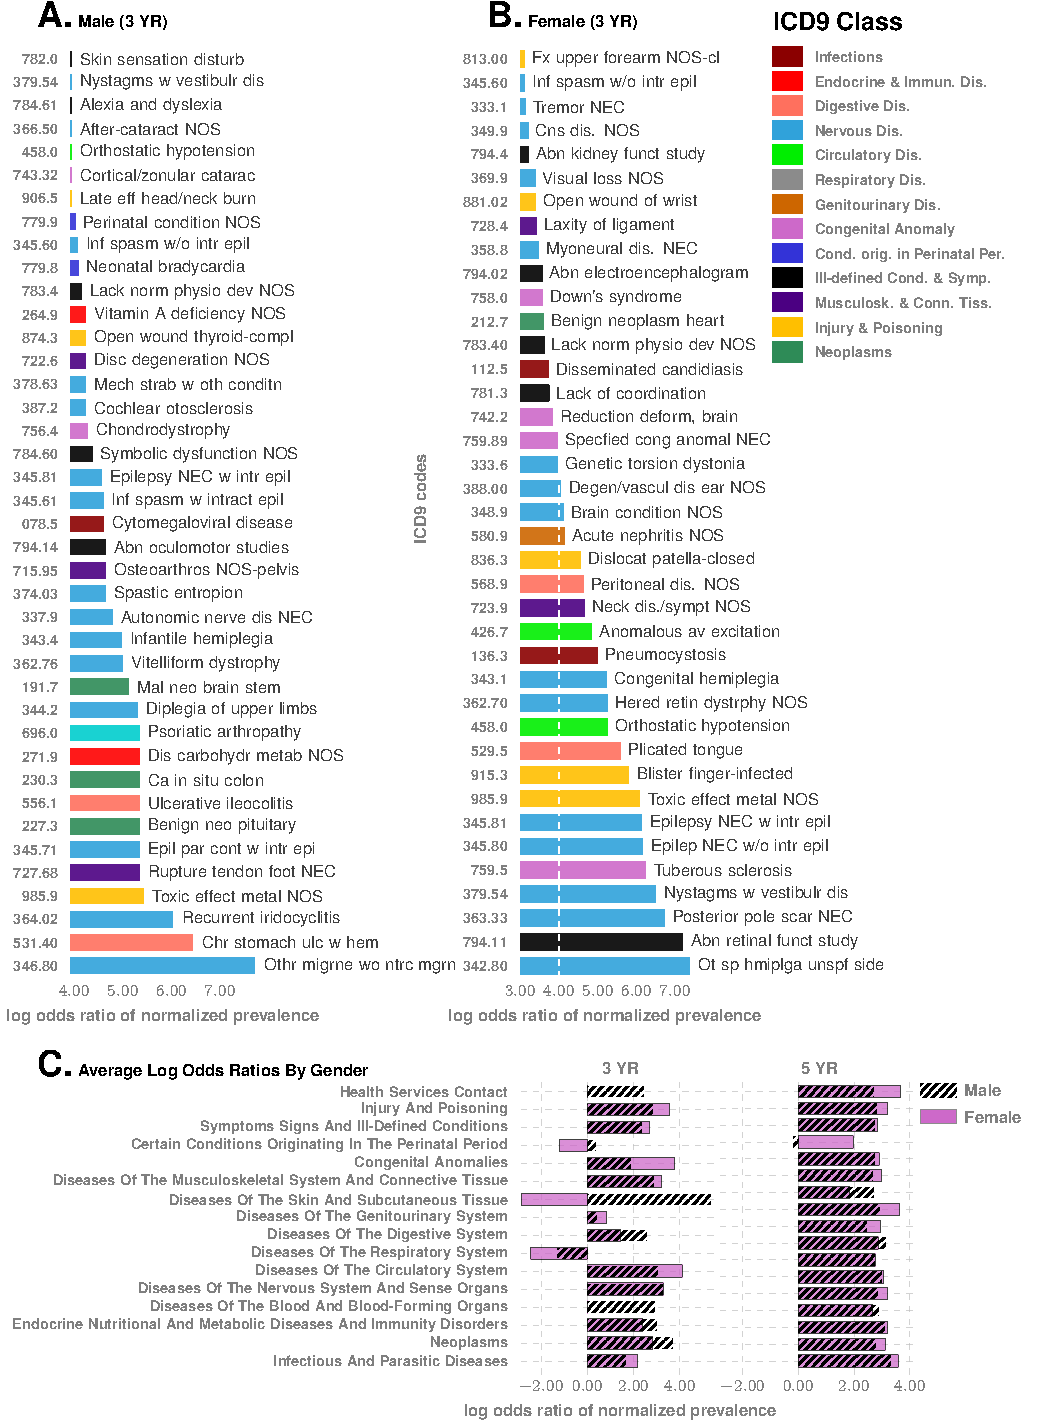
\includegraphics[width=0.99\textwidth]{Figures/External/comorbidA}
\fi
  \vspace{-5pt}
  
  \captionN{\textbf{Co-morbidity Patterns} Panel A and B. Difference in occurrence frequencies of diagnostic codes between true positive (TP) and true negative (TN) predictions. The dotted line on panel B shows the  abscissa lower cut-off in Panel A, illustrating the lower prevalence of codes in females. Panel C illustrates log-odds ratios for ICD9 disease categories at different ages. Importantly, the negative associations disappear when we consider older children, consistent with the lack of such reports in the literature which lack studies on very young cohorts. }\label{EXT-fig3}
  \vspace{-5pt}
  
\end{figure*}
\else
\refstepcounter{figure}\label{EXT-fig3}
\fi
% ###########################################################
% #############

%#################################### 
\begin{table}[!ht]
\centering

\mnp{.89\textwidth}{

\captionN{Boosted Sensitivity, Specificity and PPV Achieved at  \textbf{150 weeks}  Conditioned on M-CHAT/F Scores}\label{EXT-tabboost150}
  \vskip .5em

\begin{tabular} {L{.33in}|L{.33in}|L{.33in}|L{.33in}||L{.35in}|L{.35in}|L{.375in}||L{.375in}|L{.35in}|L{.35in}||L{.6in}}
\hline
\multicolumn{4}{c||}{\cellcolor{lightgray!60}M-CHAT/F Outcome}  & \multicolumn{3}{c||}{\mnp{.9in}{\vskip .2em global\\performance (Truven)\vskip .2em  } }&\multicolumn{3}{c||}{\mnp{1in}{\vskip .2em global\\performance\\(UCM)\vskip .2em }} &  \multirow{3}{*}{prevalence}\\\cline{0-9}
 0-2  NEG & 3-7  NEG & 3-7  POS & $\geq  8$  POS & \multirow{2}{*}{\mnp{.1in}{speci-ficity}} & \multirow{2}{*}{\mnp{.1in}{sensi-tivity}} &\multirow{2}{*}{PPV}& \multirow{2}{*}{\mnp{.1in}{speci-ficity}} & \multirow{2}{*}{\mnp{.1in}{sensi-tivity}} & \multirow{2}{*}{PPV} & \\\cline{0-3}
\multicolumn{4}{c}{\cellcolor{lightgray} specificity choices}  & & & &&&&\\\hline 
  0.28&0.66&0.93&0.97&0.95&0.64&0.224&0.95&0.577&0.206&0.022\\\hline 
0.31&0.67&0.9&0.97&0.95&0.641&0.223&0.95&0.577&0.205&0.022\\\hline 
0.54&0.86&0.97&0.99&0.98&0.494&0.361&0.98&0.393&0.31&0.022\\\hline 
0.41&0.89&0.96&0.99&0.98&0.493&0.362&0.98&0.391&0.311&0.022\\\hline 
0.31&0.61&0.86&0.98&0.95&0.808&0.219&0.95&0.713&0.198&0.017\\\hline 
0.33&0.6&0.86&0.98&0.95&0.809&0.218&0.95&0.715&0.197&0.017\\\hline 
0.66&0.95&0.98&0.99&0.98&0.574&0.337&0.98&0.417&0.269&0.017\\\hline 
0.53&0.97&0.98&0.99&0.98&0.573&0.337&0.98&0.412&0.267&0.017\\\hline 
0.54&0.91&0.97&0.99&0.978&0.615&0.322&0.978&0.499&0.278&0.017\\\hline 
0.52&0.92&0.97&0.99&0.978&0.612&0.324&0.978&0.492&0.278&0.017\\\hline 
 
\end{tabular}}

\vspace{10pt}

\mnp{.97\textwidth}{
  \captionN{Population Stratification Results on large M-CHAT/F Study(n=20,375)  reproduced from Guthrie $\etal$~\cite{pmid31562252} }\label{EXT-tabCHOP}
    \vskip .5em

  \begin{tabular}{C{.5in} | L{1.5in}|L{1in}|L{1in}|L{1in}||L{.5in}}\hline
 \bf \sffamily   Id &  \bf \sffamily Sub-population & \bf \sffamily Test Result & \bf \sffamily ASD positive & \bf \sffamily ASD Negative & \bf \sffamily Total \% \\\hline
   A &  M-CHAT/F $\geqq 8$ & Positive & 0.34\% & 0.64\% & 0.99\% \\\hline
  B &   M-CHAT/F $\in [3,7]$ & Positive (after follow-up)& 0.52\% & 4.39\% & 4.91\% \\\hline
 C &    M-CHAT/F $\in [3,7]$ & Negative (after follow-up)& 0.14\% & 3.1\% & 3.24\% \\\hline
  D &   M-CHAT/F $\in [0,2] $ & Negative & 1.22\% & 89.63\% & 90.86\% \\\hline\hline
    Total \%& &   &2.23\% & 97.77\% & 100\% \\\hline
    \end{tabular}
}

\vspace{10pt}

\mnp{.9\textwidth}{
  \captionN{$\gamma,\gamma'$ Computed from Population Stratification Recorded In  M-CHAT/F Study~\cite{pmid31562252} ($\rho=0.0223$) }\label{EXT-tabCHOP2}
    \vskip .5em

  \begin{tabular}{C{.5in} | L{1.35in} | L{1.5in}|L{.35in}|L{.35in}|L{.35in}|L{.35in}}\hline
 \bf \sffamily   Id  &  \bf \sffamily Sub-population& \bf \sffamily Test Result & $\beta_i$ & $\rho_i$ & \bf \sffamily $\gamma_i$ & \bf \sffamily $\gamma'_i$ \\\hline
   A & M-CHAT/F $\geqq 8$ &  Positive &.0099 & .3469 &.1540  & .0066 \\\hline
  B & M-CHAT/F $\in [3,7]$ & Positive (after follow-up)& .0491 & .1059 &.2331  & .0449 \\\hline
 C &   M-CHAT/F $\in [3,7]$ & Negative (after follow-up)& .0324 & .0432 &.0627  & .0317 \\\hline
  D &  M-CHAT/F $\in [0,2] $ & Negative & .9086 & .0134 &.5471  & .9168 \\\hline
    \end{tabular}}

\end{table}
%###############################################
%###############################################
